\documentclass[unicode,11pt,a4paper,oneside,numbers=endperiod,openany]{scrartcl}

% Required packages
\usepackage{amssymb} % for extended mathematical symbols
\usepackage{graphicx} % for including images
\usepackage{amsmath} % for mathematical equations
\usepackage{matlab-prettifier} % for MATLAB code snippets
\usepackage{float} % for enforcing element placement
\usepackage[export]{adjustbox} % for adjusting image placement
\usepackage{multirow} % for table cells spanning multiple rows
\usepackage{booktabs} % for better table formatting
\usepackage{algorithm} % for algorithm display
\usepackage{algpseudocode} % for pseudocode
\usepackage{physics} % for math symbols like norm, abs

\renewcommand{\thesubsection}{\arabic{subsection}}

% Macros for convenience
\newcommand{\myvec}[1]{\begin{bmatrix} #1 \end{bmatrix}}
\newcommand{\myFigure}[4]{
    \begin{figure}[htbp]
    \centering
    \caption{#1}
    \label{#2}
    \includegraphics[width=\textwidth, trim=#3]{./figures/#4}
    \end{figure}
}

\usepackage{ifthen}
\usepackage[utf8]{inputenc}
\usepackage{graphics}
\usepackage{graphicx}
\usepackage{hyperref}

\pagestyle{plain}
\voffset -5mm
\oddsidemargin  0mm
\evensidemargin -11mm
\marginparwidth 2cm
\marginparsep 0pt
\topmargin 0mm
\headheight 0pt
\headsep 0pt
\topskip 0pt        
\textheight 255mm
\textwidth 165mm

\newcommand{\duedate} {}
\newcommand{\setduedate}[1]{%
\renewcommand\duedate {\textbf{Due date:}~ #1}}
\newcommand\isassignment {false}
\newcommand{\setassignment}{\renewcommand\isassignment {true}}
\newcommand{\ifassignment}[1]{\ifthenelse{\boolean{\isassignment}}{#1}{}}
\newcommand{\ifnotassignment}[1]{\ifthenelse{\boolean{\isassignment}}{}{#1}}
\newcommand{\punkte}[1]{\hspace{1ex}\emph{\mdseries\hfill(#1~\ifcase#1{Points}\or{Points}\else{Points}\fi)}}


\newcommand\serieheader[6]{
\thispagestyle{empty}%
\begin{flushleft}

\includegraphics[width=0.45\textwidth]{usi-inf-logo.pdf}
\end{flushleft}
  \noindent%
  {\large\ignorespaces{\textbf{#1}}\hspace{\fill}\ignorespaces{ \textbf{#2}}}\\ \\%
  {\large\ignorespaces #3 \hspace{\fill}\ignorespaces #4}\\
  \noindent%
  \bigskip
  \hrule\par\bigskip\noindent%
  \bigskip {\ignorespaces {\Large{\textbf{#5}}}
  \hspace{\fill}\ignorespaces \large \ifthenelse{\boolean{\isassignment}}{\duedate}{#6}}
  \hrule\par\bigskip\noindent%  \linebreak
}

\makeatletter
\def\enumerateMod{\ifnum \@enumdepth >3 \@toodeep\else
      \advance\@enumdepth \@ne
      \edef\@enumctr{enum\romannumeral\the\@enumdepth}\list
      {\csname label\@enumctr\endcsname}{\usecounter
        {\@enumctr}%%%? the following differs from "enumerate"
	\topsep0pt%
	\partopsep0pt%
	\itemsep0pt%
	\def\makelabel##1{\hss\llap{##1}}}\fi}
\let\endenumerateMod =\endlist
\makeatother




\usepackage{textcomp}






\begin{document}

\setassignment

\serieheader
{Computer Graphics}
{2024}
{\textbf{Students:} Davide Frova, Jamila Oubenali}
{}
{Bonus Assignment | Spatial Data Structures}{}

\section{Overview}
In this report, we detail our implementation of spatial data structures to accelerate rendering tasks for large meshes. The assignment required implementing two versions: one using bounding boxes (Version A) and another using a kd-tree (Version B). The results highlight the significant performance improvement achieved with the kd-tree approach.

\section{Implementation Details}

\subsection{Version A: Bounding Boxes}
Version A implemented a bounding box approach for spatial partitioning. This provided a moderate acceleration by reducing the number of unnecessary intersection tests during rendering. However, the linear processing of bounding box content remained a bottleneck for large meshes.

\subsection{Version B: kd-Tree}
Motivated by the inefficiencies in Version A, we implemented a kd-tree for Version B. The kd-tree was chosen for its efficient hierarchical partitioning, which allows for fast traversal. We configured the kd-tree with a leaf size of 5 elements, balancing tree depth and traversal cost.

The results were remarkable: the kd-tree drastically reduced rendering times, making it possible to handle meshes with millions of triangles. This significant improvement underscores the importance of effective spatial data structures for complex scenes.

\section{Results and Discussion}
To evaluate the effectiveness of kd-tree acceleration (Version B) compared to no acceleration, we analyzed render times for four different scenarios with increasing numbers of triangles: the Bunny, Armadillo, Lucy, and a combined scene (all three meshes). The render times and triangle counts are summarized below:

\begin{table}[H]
    \centering
    \begin{tabular}{lccc}
        \toprule
        \textbf{Mesh}  & \textbf{\# of Triangles} & \textbf{Render Time (No Acc)} & \textbf{Render Time (kd-tree)} \\
        \midrule
        Bunny          & 1,392                    & 90.93 seconds                 & 0.59 seconds                   \\
        Armadillo      & 3,112                    & 229.46 seconds                & 0.83 seconds                   \\
        Lucy           & 2,804                    & 199.99 seconds                & 0.87 seconds                   \\
        All (Combined) & 7,308                    & 868.34 seconds                & 1.53 seconds                   \\
        \bottomrule
    \end{tabular}
    \caption{Rendering time comparison for no acceleration vs kd-tree acceleration.}
    \label{tab:results}
\end{table}

\subsubsection*{Plot Analysis}
Figures \ref{fig:comparison-linear} and \ref{fig:comparison-log} visualize the performance comparison.
\\
\textbf{Linear Scale (Figure \ref{fig:comparison-linear})}: The kd-tree acceleration significantly reduces render times compared to the no-acceleration version, particularly as the number of triangles increases. For example, the render time for the combined scene drops from 868 seconds to just 1.53 seconds.
\\
\textbf{Logarithmic Scale (Figure \ref{fig:comparison-log})}: On a logarithmic scale, the trend highlights the exponential growth in render times for the unoptimized version compared to the near-linear growth for the kd-tree implementation. This confirms the scalability of the kd-tree for large datasets.

\begin{figure}[H]
    \centering
    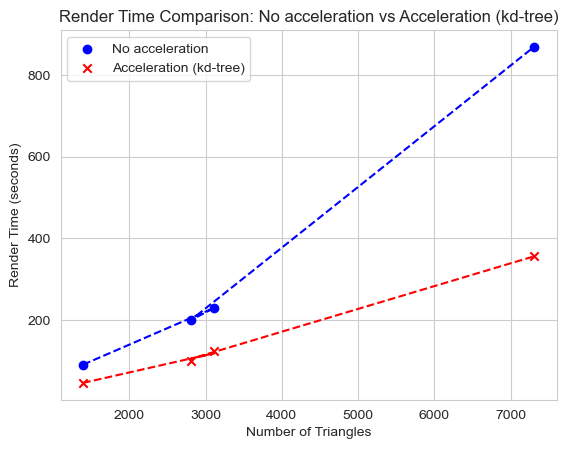
\includegraphics[width=\textwidth]{comparison.png}
    \caption{Rendering time comparison: No acceleration vs. kd-tree acceleration.}
    \label{fig:comparison-linear}
\end{figure}

\begin{figure}[H]
    \centering
    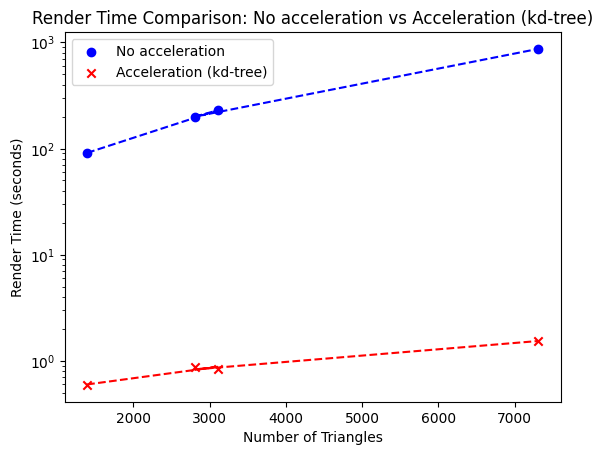
\includegraphics[width=\textwidth]{comparison_log.png}
    \caption{Rendering time comparison: No acceleration vs. kd-tree acceleration (logarithmic scale).}
    \label{fig:comparison-log}
\end{figure}

\subsection{High-Resolution Meshes with Shadows Enabled}
While the above comparisons were based on low-resolution meshes with shadows disabled, we also tested the kd-tree implementation on a full-resolution scene with shadows enabled. The scene included the following properties:
\begin{itemize}
    \item \textbf{Meshes}:
          \begin{itemize}
              \item \textbf{Armadillo}
                    \begin{itemize}
                        \item \textbf{Number of Triangles}: 345,944
                        \item \textbf{Number of Vertices}: 172,974
                    \end{itemize}
              \item \textbf{Bunny}
                    \begin{itemize}
                        \item \textbf{Number of Triangles}: 69,451
                        \item \textbf{Number of Vertices}: 35,947
                    \end{itemize}
              \item \textbf{Lucy}
                    \begin{itemize}
                        \item \textbf{Number of Triangles}: 2,805,572
                        \item \textbf{Number of Vertices}: 1,402,794
                    \end{itemize}
          \end{itemize}
    \item \textbf{Total Number of Triangles}: 3,220,967
    \item \textbf{Total Number of Vertices}: 1,611,715
\end{itemize}

The results were impressive:
\begin{itemize}
    \item Time to define the scene (building kd-tree included): \textbf{13.41 seconds}.
    \item Time to render the image: \textbf{18.28 seconds}.
\end{itemize}

These results demonstrate the kd-tree's scalability, even when rendering scenes with millions of triangles and computationally expensive features such as shadows.

\subsubsection*{Key Observations}
1. \textbf{Drastic Speedup}: The kd-tree reduced render times by 2-3 orders of magnitude for low-resolution meshes and maintained exceptional performance for high-resolution scenes.
\\
2. \textbf{Scalability}: The kd-tree handled a full scene with over 3.2 million triangles and shadows enabled, demonstrating its scalability for highly complex scenes.
\\
3. \textbf{Low Overhead}: For low-resolution meshes, the kd-tree maintained sub-second render times, even for moderately complex scenes.

\section{Future Optimizations}
One potential optimization is to explore a balance between the kd-tree's leaf size and introducing a Bounding Volume Hierarchy (BVH) for processing leaf nodes. Currently, leaf nodes are processed linearly, which may still become a bottleneck for highly complex meshes. Implementing a BVH within the leaf nodes could further improve traversal efficiency.

\section{Conclusion}
The implementation of the kd-tree (Version B) demonstrated a dramatic improvement in performance compared to the bounding box approach (Version A). The kd-tree scaled efficiently, handling both low-resolution meshes and high-resolution scenes with millions of triangles. While further optimizations, such as BVH integration, remain as potential future work, the kd-tree has proven to be a highly effective spatial data structure for complex rendering tasks.

\end{document}
